\section{Problem Formulation}
\label{sec:problem}

In this section, we formally introduce our three unsupervised automata learning problems and prove that the first two are computationally hard.
As mentioned in the introduction, all three learning settings are assumed to be given a sample $\mathcal{S}$ of unlabeled words.
The first setup, which we refer to as \emph{Two-Bound DFA Learning}, additionally requires being given two natural numbers $\ell,u \in \mathbb{N}$ with $\ell \leq u \leq \abs{\sample}$.
While the precise labels of the words in the sample $\mathcal{S}$ are unknown, these numbers provide an estimate of the distribution of positive words in $\mathcal{S}$.
Then, the task is to learn a minimal DFA which accepts at least $\ell$
and at most $u$ words from $\mathcal{S}$.
We formally state this problem as:
\begin{problem}[Two-Bound DFA Learning Problem]
\label{problem:1}\\
Given a multi-set of words $\sample~=~\{w_1, \dots, w_n\}$ and two natural
numbers $\ell,u \in \mathbb{N}$ with $\ell \leq u \leq \abs{\sample}$, construct a DFA $\dfa$ which accepts at least $\ell$ and at most $u$ words
from $\sample$.
\end{problem}

Notice that one may not always find a solution for this problem.
This is illustrated using the following example.
\begin{example}
Consider the bounds $\ell = u = 1$ and the sample $\sample$ which only contains the word $'a'$ twice.
Being deterministic, every DFA has to either accept both copies of the word $'a'$ or reject them both.
Hence there does not exist a DFA fulfilling the bounds in this case. 
\end{example}

%This is illustrated using the following example.
%\begin{example}
%Consider the bounds $\ell = u = 1$ and the sample $\sample$ which only contains the word $'a'$ twice.
%Being deterministic, every DFA has to either accept both copies of the word $'a'$ or reject them both.
%Hence there does not exist a DFA fulfilling the bounds in this case. 
%\end{example}
Despite this, Problem~\ref{problem:1} is decidable.
To show decidability, we first represent the sample as a \emph{prefix tree}~\cite{de2010grammatical}.
A prefix tree for a sample $\sample$ is a partial DFA (i.e., some transitions are unspecified) without final states such that, after reading a word $w \in \sample$, the DFA is in a unique state $q_w$.
An example of a prefix tree is displayed in Figure~\ref{fig:pt}.
We complete this partial DFA by adding an additional sink state that becomes the target of all unspecified transitions.
To decide whether there exists a DFA accepting at least $\ell$ and at most $u$ words, we iterate over all combinations of final states and check the number of accepted words in each case.
Since there is a unique state for each word in $\sample$, either one of these DFAs fulfills the bounds or we can conclude that none exists.
%
\begin{figure}
    \centering
    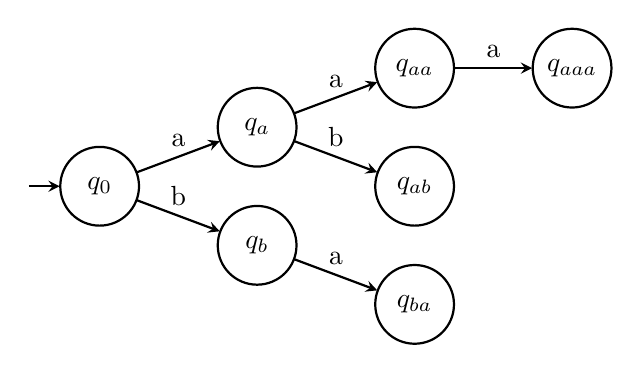
\begin{tikzpicture}[scale=0.5]
        \draw[thick] (0,0) circle (1);
        \node[circle, minimum size = 10mm] (0) at (0,0) {$q_0$};
        
        \draw[thick] (4,1.5) circle (1);
        \node[circle, minimum size = 10mm] (a) at (4,1.5) {$q_{a}$};
        
        \draw[thick] (4,-1.5) circle (1);
        \node[circle, minimum size = 10mm] (b) at (4,-1.5) {$q_{b}$};
        
        \draw[thick] (8,3) circle (1);
        \node[circle, minimum size = 10mm] (aa) at (8,3) {$q_{aa}$};
        
        \draw[thick] (8,0) circle (1);
        \node[circle, minimum size = 10mm] (ab) at (8,0) {$q_{ab}$};
        
        \draw[thick] (8,-3) circle (1);
        \node[circle, minimum size = 10mm] (ba) at (8,-3) {$q_{ba}$};
        
        \draw[thick] (12,3) circle (1);
        \node[circle, minimum size = 10mm] (aaa) at (12,3) {$q_{aaa}$};
        
        \draw[thick, -{stealth}] (-1.8,0) -- (0);
        \draw[thick, -{stealth}] (0) -- (a) node [midway, above] {a};
        \draw[thick, -{stealth}] (0) -- (b) node[midway,above]{b};
        \draw[thick, -{stealth}] (a) -- (aa) node[midway,above]{a};
        \draw[thick, -{stealth}] (a) -- (ab) node[midway,above]{b};
        \draw[thick, -{stealth}] (b) -- (ba) node[midway,above]{a};
        \draw[thick, -{stealth}] (aa) -- (aaa) node[midway,above]{a};
    
    \end{tikzpicture}
    \caption{Prefix tree for the sample $(aa, ab, ba, aaa)$}
    \label{fig:pt}
\end{figure}
%
However, a DFA constructed this way will generally be unsuitable for applications such as anomaly detection as it suffers from two main issues.
On the one hand, by design, it overfits the sample $\sample$ and thus poorly generalizes to unseen data.
On the other hand, it becomes rather large, hindering interpretability in the sense of Occam's razor.
To overcome these issues, we propose an algorithm that constructs a DFA of \emph{minimal size} fulfilling the given bounds (if one exists).
By requiring minimality, however, the problem becomes computationally hard.
In fact, it can be shown that the problem of whether there exists a DFA
with $n$ states for Problem \ref{problem:1} is \NP-complete. 

\begin{theorem}
\label{thm:NP-complete}
	Given a multi-set of words $\sample$, two natural numbers
	$\ell,u \in \mathbb{N}$ with $\ell \leq u \leq \abs{\sample}$,
	and a natural number $n$ (given in unary), the problem of finding
	a DFA $\dfa$ with $n$ states that accepts at least
	$\ell$ and at most $u$ words from $\sample$ is \NP-complete.
\end{theorem}

In order to prove Theorem~\ref{thm:NP-complete}, we begin by showing that the problem is in \NP, as formalized in the following Lemma.

    \begin{lemma}
    \label{thm:NP}
        Given a multi-set of words $\sample$, two natural numbers $\ell,u \in \mathbb{N}$ with $\ell \leq u \leq \abs{\sample}$, and a natural number $n$ (given in unary), a non-deterministic Turing machine can compute in polynomial time whether there exists a DFA $\dfa$ with $n$ states which accepts at least $\ell$ and at most $u$ words from $\sample$ (i.e., the problem lies in \NP).
    \end{lemma}

    \begin{proof} [of Lemma~\ref{thm:NP}]
    	Let $\sample,\ell,u,$ and $n$ be given.
        As $n$ is unary, a non-deterministic Turing machine can guess an automaton $\dfa$ with $n$ states.
        The number of accepted words from $\sample$ can then be computed in polynomial time by simulation.
        Finally, checking whether this number is at least $\ell$ and at most $u$ is also possible in polynomial time, showing that the problem lies in \NP. \qed
    \end{proof}

Next, we we show \NP-hardness of Problem~\ref{problem:1}, thus we conclude that it is \NP-complete.
    
    \begin{lemma}
    \label{thm:NP-hard}
    	Given a multi-set of words $\sample$, two natural numbers $\ell,u \in \mathbb{N}$ with $\ell \leq u \leq \abs{\sample}$, and a natural number $n$ (given in unary), the problem of finding a DFA $\dfa$ with $n$ states which accepts at least $\ell$ and at most $u$ words from $\sample$, is \NP-hard.
    \end{lemma}

    To proof Lemma~\ref{thm:NP-hard}, we use the \NP-completeness of the following problem (see \cite{DBLP:books/fm/GareyJ79}).

    \begin{problem}\label{problem:NP-Complete}
    	Given finite disjoint sets of words $P,N\subseteq\Sigma^*$ and a unary number $k\in\mathbb{N}_0$, does there exist a deterministic finite automaton $\dfa$ with $k$ states such that $\dfa$ accepts all words in $P$ and rejects all words in $N$.
    \end{problem}

    As detailed in the proof below, \NP-hardness (and thus \NP-completeness) of our problem follows by reduction from Problem \ref{problem:NP-Complete}.
    This reduction makes use of the multi-set structure of the samples to encode positive and negative words from Problem \ref{problem:NP-Complete} in different multiplicities in the multi-set, which can be distinguished by Problem \ref{problem:1}.

    \begin{proof} [of Lemma~\ref{thm:NP-hard}]
    	We show this by a many-one reduction from Problem \ref{problem:NP-Complete}.
    	Let finite disjoint sets $P,N\subseteq\Sigma^*$ and a unary number $k\in\mathbb{N}_0$ be given.
    	We construct an instance of our problem as follows:
        \begin{itemize}
            \item $n\coloneqq k$;
            \item $\sample(w)\coloneqq\begin{cases}
                                    \abs{N}+1&\text{if }w\in P,\\
                                    1&\text{if }w\in N,\\
                                    0&\text{otherwise,}
            \end{cases}$
    
    		for $w\in\Sigma^*$, i.e., the multi-set contains
    		exactly $(\abs{N}+1)$-times all words in $P$ and once all
    		words in $N$;
            \item $\ell=u\coloneqq\abs{P}(\abs{N}+1)$.
        \end{itemize}
        This construction can be done in polynomial time.
    
        Furthermore, if there exists a DFA $\dfa$ with $n$ states solving Problem \ref{problem:1} for $\sample,\ell,$ and $u$ as above, i.e., accepting exactly $\abs{P}(\abs{N}+1)$ words from $\sample$, we have that
        \[
        0\equiv\sum_{w\in P\cup N}\sample(w)\cdot\dfa(w)\equiv\sum_{w\in N}\dfa(w)\pmod{\abs{N}+1}
        \]
        Recall that $\sample(w)$ denotes the number of occurrences of $w$ in $\sample$ and $\dfa(w)$ indicates whether $w$ is accepted by $\dfa$.
    	This shows that $\dfa$ rejects all words in $N$, and, thus
        \[
        \abs{P}(\abs{N}+1)=\sum_{w\in P}\sample(w)\cdot\dfa(w)\Rightarrow\abs{P}=\sum_{w\in P}\dfa(w),
        \]
        showing that $\dfa$ accepts all words in $P$ whence $\dfa$ is also a solution to the instance $(P,N,k)$ of Problem \ref{problem:NP-Complete}.
    
        Similarly, if there exists a DFA $\dfa$ solving the instance $(P,N,k)$ of Problem \ref{problem:NP-Complete}, we have that
        \[
        \sum_{w\in\Sigma^*}\sample(w)\cdot\dfa(w)=(\abs{N}+1)\sum_{w\in P}\dfa(w)=\abs{P}(\abs{N}+1),
        \]
        whence $\dfa$ is also a solution with $n$ states to the instance $(\sample,\ell,u)$ of Problem \ref{problem:1}.
    
        All in all, this shows the reduction from Problem \ref{problem:NP-Complete}, and thus \NP-hardness of finding a solution of Problem \ref{problem:1} with $n$ states. \qed
    \end{proof}

%\NP-completeness of Problem~\ref{problem:1} follows from it being in \NP and being \NP-hard.

In this first setup, we require the user to provide a lower and an upper bound on the distribution of positive words in a given sample.
However, in practice, this requirement may be too strong.
Thus, in the second setup, which we refer to as \emph{Single-Bound DFA Learning}, 
we reduce the amount of prior knowledge compared to the first case by removing requirement to specify both $\ell$ and $u$.
Instead, we assume to be given only one parameter, say $\ell$ (the case in which $u$ is given is analogous).
Now, in contrast to Problem~\ref{problem:1}, the task to construct a minimal DFA that accepts at least $\ell$ words from $\sample$ always has a trivial solution: the DFA that accepts all words in $S$ only has size 1 and fulfills the bound.
However, this DFA underfits the sample $\sample$ and thus does not capture the underlying structure.
To reduce underfitting, we apply a common technique from automata learning and construct a DFA of a fixed size that accepts the smallest number $k \geq l$ of words from the sample. 
By providing this size as an additional parameter $n$ the user can regularize the trade-off between avoiding underfitting (larger) and interpretability (smaller).
We formally state this problem as:
\begin{problem}[Single-Bound-Learning-Problem]
\label{problem:2}\\
Given a multi-set of words $\sample = \{w_1, \dots, w_n\}$ and two natural numbers $\ell, n \in \mathbb{N}$ with $\ell \leq \abs{\sample}$, construct a DFA $\dfa$ of size $n$ which accepts the smallest number $k \geq l$ of words from $\sample$.
\end{problem}
This problem is the optimization version of Problem~\ref{problem:1}, thus, it is also computationally hard.
In fact, from Problem~\ref{problem:1} being \NP-complete, it immediately follows that Problem~\ref{problem:2} lies within the complexity class \NPO (i.e., the class of optimization problems whose decision variant lies in \NP).

The third setup, which we refer to as \emph{Distance-Based DFA Learning}, is motivated by the assumption that for many applications, the pairs of positive (or negative) words are structurally similar, resulting in a low edit distance.
In contrast, opposite classifications (i.e, one positive and one negative word) are drastically different, resulting in a high edit distance.
In the context of anomaly detection, for instance, deep learning based methods follow this idea and classify new data based on the distance to the training data (e.g.,~\cite{pmlr-v80-ruff18a}).
This assumption allows us to alleviate the user’s burden to specify any bounds.
Instead, along with the sample $\sample$, we only rely on the size $n \in \mathbb N$ of the automata as a regularizer (similar to the second setting) and a distance function over words (in our case, the Levenshtein distance).
The task is then to construct a DFA of size $n$ such that the distance between all pairs of two accepted (rejected) words is minimized while the distance between pairs of both one accepted and one rejected word is maximized.
This dual optimization problem can then be transformed into a plain minimization problem by multiplying the distances to be maximized by $-1$.
This allows us to formally state this problem as:
\begin{problem}[Distance-Based-Learning-Problem]
\label{problem:3}\\
Given a multi-set of words $\sample = \{w_1, \dots, w_n\}$ and a natural number $n \in \mathbb{N}$, construct a DFA $\dfa$ of size $n$ which minimizes the following objective function:
\begin{align}
    \sum\limits_{w_i, w_j \in L(\dfa) \cap \sample} dist(w_i, w_j)  - \sum\limits_{\substack{w_i \in L(\dfa) \cap \sample \\ w_j \notin L(\dfa) \cap \sample}} dist(w_i, w_j) \label{eq:distance}
\end{align}
where $dist(w_i, w_j)$ denotes the Levenshtein distance between two words $w_i$ and $w_j$.
\end{problem}

While we conjecture that this problem is also computationally hard, we leave a proof of its complexity as part of future work.


